\documentclass{article}

\usepackage{graphicx}
\usepackage{tikz}
\usepackage{tikzsymbols}
\usetikzlibrary{calc,patterns,shapes.geometric}
\pagestyle{empty}
\usepackage[margin=0pt]{geometry}
\geometry{papersize={14in,12in}}

\def\centerarc[#1](#2)(#3:#4:#5){\draw[#1] ($(#2)+({#5*cos(#3)},{#5*sin(#3)})$) arc (#3:#4:#5);}

\begin{document}
	\begin{figure}
		\centering
		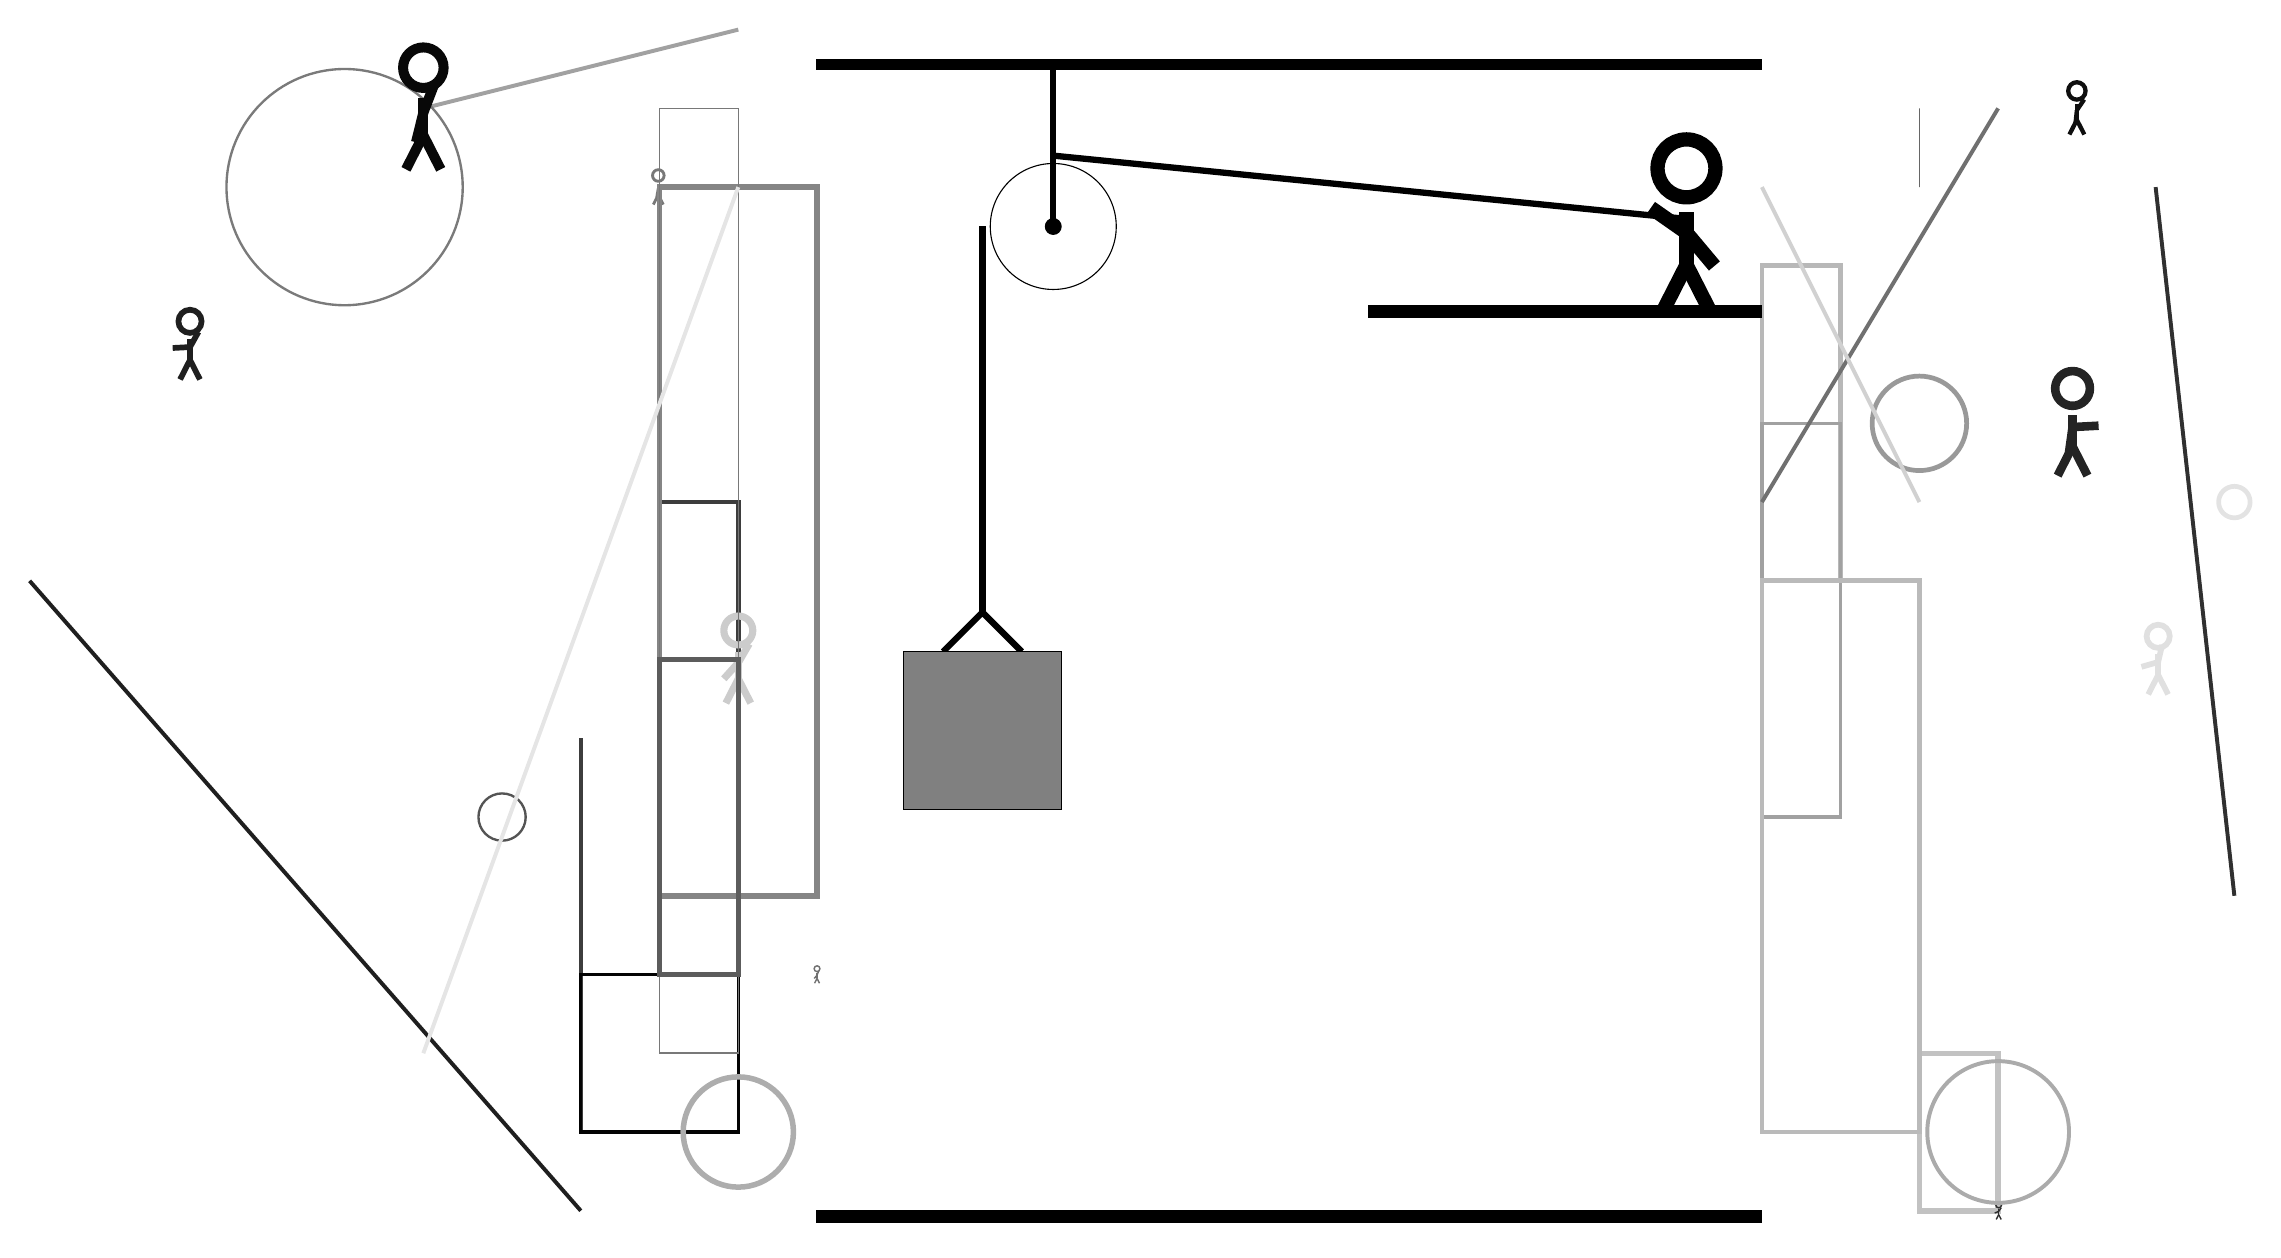
\begin{tikzpicture}
			%%%%% START %%%%%
			
			\draw[fill=black] (-2, 11.5) rectangle (10, 11.625);
			
			\draw (1, 9.5) circle (0.8);
			\draw[fill=black] (1, 9.5) circle (0.1);
			\draw[line width=0.8mm] (1, 11.5) -- (1, 9.5);
			
			\draw[line width=0.5mm, color=black!76](-5, -2) -- (-5, 3);
			
			\draw[line width=0.5mm, color=black!88](-5, -3) -- (-12, 5);
			\draw [line width=0.6mm, color=black!40](12, 7) circle (0.6);
			\draw[line width=0.4mm, color=black!99] (-3, -2) rectangle (-5, 0);
			\draw[line width=0.6mm, color=black!28] (10, 9) rectangle (11, 5);
			\draw[line width=0.5mm, color=black!37](-7, 11) -- (-3, 12);
			\draw[line width=0.6mm, color=black!76] (-3, 0) rectangle (-4, 6);
			
			\draw [line width=0.7mm, color=black!32](-3, -2) circle (0.7);
			\node[line width=0.6mm, color=black!53] at (-4, 10) {\Strichmaxerl[2][80][17]};
			\node[line width=0.3mm, color=black!20] at (-3, 4) {\Strichmaxerl[5][48][60]};
			\node[line width=0.6mm, color=black!12] at (15, 4) {\Strichmaxerl[4][16][77]};
			\draw[line width=0.7mm, color=black!48] (-4, 1) rectangle (-2, 10);
			\node[line width=0.7mm, color=black!94] at (14, 11) {\Strichmaxerl[3][84][56]};
			\draw[line width=0.2mm, color=black!53] (-3, 11) rectangle (-4, -1);
			\node[line width=0.6mm, color=black!56] at (-2, 0) {\Strichmaxerl[1][50][68]};
			\draw [line width=0.6mm, color=black!11](16, 6) circle (0.2);
			\draw[line width=0.4mm, color=black!37] (10, 7) rectangle (11, 2);
			\node[line width=0.2mm, color=black!88] at (-10, 8) {\Strichmaxerl[4][3][61]};
			\node[line width=0.7mm, color=black!86] at (14, 7) {\Strichmaxerl[6][82][3]};
			\draw [line width=0.3mm, color=black!52](-8, 10) circle (1.5);
			\draw[line width=0.7mm, color=black!24] (12, -3) rectangle (13, -1);
			\draw[line width=0.6mm, color=black!64] (-3, 4) rectangle (-4, 0);
			\draw[line width=0.5mm, color=black!56](13, 11) -- (10, 6);
			\node[line width=0.7mm, color=black!82] at (13, -3) {\Strichmaxerl[1][23][55]};
			\draw [line width=0.5mm, color=black!33](13, -2) circle (0.9);
			\draw[line width=0.5mm, color=black!81](15, 10) -- (16, 1);
			
			\draw[line width=0.6mm, color=black!27] (12, -2) rectangle (10, 5);
			\draw[line width=0.5mm, color=black!18](10, 10) -- (12, 6);
			\draw [line width=0.3mm, color=black!84](-3, 1) circle (0.0);
			\draw[line width=0.2mm, color=black!60] (12, 10) rectangle (12, 11);
			\draw [line width=0.3mm, color=black!67](-6, 2) circle (0.3);
			
			\draw[line width=0.5mm, color=black!10](-7, -1) -- (-3, 10);
			\node[line width=0.4mm, color=black!97] at (-7, 11) {\Strichmaxerl[7][76][69]};
			
			\draw[line width=0.8mm](-0.4, 4.1) --  (0.1, 4.6) -- (0.6, 4.1);
			\draw[fill=black!50] (-0.9, 4.1) rectangle (1.1, 2.1);
			
			\draw[line width=0.8mm](0.1, 9.5) -- (0.1, 4.6);
			\centerarc[line width=0.8mm](1, 9.5)(90:180:0.9)
			\draw[line width=0.8mm](1, 10.4) -- (9, 9.6);
			
			\node at (9, 9.5) {\Strichmaxerl[10][-35][-50]};
			\draw[fill=black] (5, 8.5) rectangle (10, 8.35);
			
			\draw[fill=black] (-2, -3) rectangle (10, -3.15);
			
			%%%%% END %%%%%
		\end{tikzpicture}
	\end{figure}	
\end{document}